\documentclass[conference]{IEEEtran}
\usepackage{graphicx}
\usepackage{soul}
\usepackage{todonotes}
\usepackage{amsmath}
\usepackage{algorithm}
\usepackage{algpseudocode}

\begin{document}

\title{Design of Fine-grained Sequential Approximate Circuits using Probability-aware Fault Emulation}


\author{\IEEEauthorblockN{BLIND REVIEW}
\IEEEauthorblockA{}
\and
\IEEEauthorblockN{BLIND REVIEW}
\IEEEauthorblockA{}
}


% make the title area
\maketitle


\begin{abstract}
%\boldmath
Approximate Computing has recently drawn interest due to its promise to substantially decrease the power consumption of integrated circuits. By tolerating a certain imprecision at a circuit output, it can be operated at a more resource-saving state. For instance, parts of the circuit could be switched off or driven at sub-threshold voltage. Clearly, not all applications are suitable for this approach. Especially applications from the signal and image processing domain are applicable, due to their intrinsic tolerance to imprecision. But even in these circuits, one has to be very careful where to approximate a circuit and to what extent, in order not to violate a minimum required QoS.\\
In this paper we are presenting an approach to generate approximate circuits from existing deterministic implementations. The flow reaches from application-driven QoS definition down to approximated RTL. We are employing FPGA-based fault emulation of the circuit in order to find out how faults, i.e. imprecisions in the circuit, affect the circuit behavior.\\
Most existing approaches only consider combinational circuits. Our proposed methodology is able to approximate complete sequential circuits. Due to the FPGA-based emulation, our approach is very fast and accurate. And furthermore, it allows us to fine-granular tune the resulting precision to the defined QoS, in order to bring out the best gain of the approximation.
\end{abstract}

\IEEEpeerreviewmaketitle



\section{Introduction}
Due to the increasing demand for low-power applications during the last decade, energy-efficiency has become a major concern in embedded systems design. However, voltage-scaling, the most efficient technique to save power, can not be further driven in conventional systems. Apart from a not acceptable performance loss, the aggressive scaling of \mbox{MOSFET} feature-sizes, makes circuits prone to even small voltage variations, when operating in the near-threshold area and hence susceptible to errors within the circuit.
\subsubsection*{Approximate Computing}
One emerging approach to tackle this problem is captioned by the term \emph{Approximate Computing}. Approximate computing tries to increase the energy-efficiency by tolerating a certain uncertainty at the circuit outputs, i.e. the result of a operation. The term covers a variety of points of application, from programming level to transistor level, as well as techniques on how to reduce the power consumption. Power can be saved for instance by calculating with a \emph{reduced precision}, i.e. removing parts of the circuit, a method clearly related to fixed-point arithmetic. However, approximate computing introduces dynamics to this field. It proposes to switch off and on the precision depending on the actual demand of the application. Another way can be to \emph{over-scale the voltage}, and hence accept timing violations or nose-based faults. 
%Another method, we want to explicitly mention here, is related to circuit soft-error reliability. Approximate computing can be used to reduce the hardware overhead due to fault tolerance mechanisms, e.g. by \emph{omitting redundancy} wherever it is not absolutely needed.
Clearly, this approach is not applicable for all kind of applications. Especially applications from the signal processing domain are suitable. These applications usually have an inherent imprecision tolerance. They have to deal with the human (imperfect) perception, have redundant input data in order to deal with noisy data. For a comprehensive coverage of the topic, we refer to the work of Han et al. \cite{han_approximate_2013}.
\subsubsection*{Motivational Example}
Consider any arbitrary wireless communication system, e.g. like IEEE 802.11 Wi-Fi. Like any similar system, 802.11 is as system, designed to deal with noise on the received radio signal. It is designed to transmit data in good, as well as bad communication channel. If the channel is noisy between two stations, the some systems switch to a lower-order modulation scheme, resulting in a lower data-rate, in order to be more robust. However, internally the hardware is working with the same precision independent on the signal quality, which might not be necessary. For instance, such systems usually consist of one or more channel-coding schemes. Ideally, at the receiving end, the payload is extracted from the received signal, not matter if it was noisy or not. Hence, if the SNR of the signal is high, the decoder could work less precise, requiring less power, and still extract the payload error-free. Depending on the signal quality such a dynamic approximate system could then switch between different power/precision states without having any influence on the performance.
\subsubsection*{Problem Description}
Even if the applications mentioned above seem to be applicable for approximate computing, parts of the circuit cannot be easily switched off and faults cannot be tolerated everywhere in the circuit. It is crucial to know which parts of the circuit influence the functionality in which way. Ideally, we want to gain this knowledge for each gate in the circuit, to get a very detailed overview about the possible approximations. To simplify the problem we are considering circuits at register-transfer level, which gives us a good trade-off between the precision of gate-level and the abstraction of algorithmic level. However, even there the number of possible states of the circuit corresponds to $2^N$, where $N$ is the number of registers in the circuit. Hence, the difficulty of designing approximate computing on circuit level is to efficiently and reliable determine which parts of the circuit can be approximated and to what extent.
\subsubsection*{Related Work}
As mentioned earlier, approximate computing is a research field that can, and in our opinion has be, considered at many levels. Furthermore, it can be applied to CPU based applications, as well as dedicated hardware accelerators. In the former case usually the source code is annotated defining which operations can be executed on approximate hardware, e.g. as proposed in \cite{sampson_enerj:_2011}. In the latter case, most research effort has been spend on building approximate standard building blocks, like adders and multipliers \cite{huang_exploring_2011,chakrapani_highly_2008,gupta_impact:_2011,kahng_accuracy-configurable_2012}. However, most methods presented are based on manual interaction. Only a few present an automated approach, like Nepal et al., who proposed an automated method, based on the behavioral description. Some works focus on approximation of integrated circuits at synthesis time \cite{miao_approximate_2013,shin_approximate_2010,choudhury_approximate_2008}. However, only very few explicitly focus on the approximation of sequential circuits. Ranjan et al. \cite{ranjan_aslan:_2014} use formal verification techniques to identify the impact of approximate parts of a sequential circuit on the global output. This seems to be a very promising approach. However, it only offers the ability to generate fixed approximated circuits. In order to save power e.g. by using dynamic voltage over-scaling or by dynamically enabling precision, an even more fine-grained analysis is required, to model varying approximation operating points.
\subsubsection*{Contribution of this Work}
In order to solve these limitations we are introducing bit-flip probabilities to the analysis. As already mentioned, we are focusing on register-transfer level. By assigning bit-flip probabilities to each register in a circuit, we are able to model the various effects responsible for the approximation, from timing violations to circuit pruning. We are using FPGA-based emulation to actually flip the bits. This makes the analysis very fast and allows us to cover a large state space, so that the results are reliable. In this work we are presenting and evaluating a methodology in order to find out which parts of a sequential circuit can be approximated and to what extent. The approach is automated wherever it is possible. Given a netlist and a set of quality constraints our tool automatically generates the information of what bit-flip probability is allowed at which register, without violating the output constraint. The approach is fine-granular. I.e. we can not only model the ``integer'' pruning of circuit elements, but also model a bit-flip probability. Integer approximations, i.e. if parts of the circuit can be pruned, can then be implemented directly. Non-integer information can then be used generate approximate combinational logic, e.g. based on aggressive power-scaling, using existing solutions.

The remainder of this paper is organized as follows: In Section \ref{sec:methodology} we are explaining our methodology in detail. In Section \ref{sec:experimental_results} we will evaluate our approach with various realistic benchmark circuits and compare the performance with other approaches. And finally, in Section \ref{sec:conclusion} we will conclude our work.





\section{Methodology}
\label{sec:methodology}
\subsection{Probability-aware Fault Emulation}
%\begin{figure}[htb]
%  \centering
%  \missingfigure[figwidth=.5\textwidth]{Simulator block-diagram}
%  \caption{Block-diagram of the FPGA-based fault emulation system}
%  \label{fig:faultify_block}
%\end{figure}
In our previous work we have developed an FPGA-based fault emulation system. In this work, we are using this system to detect which parts of a circuit can be approximated. Emulation means, that the circuit we want to approximate is mapped on an FPGA, independent on the target architecture. To make the emulation as realistic as possible, the circuits have to be emulated, after being synthesized for the specific target technology. In case of an ASIC target, primitives of the ASIC library have to be replaced by corresponding FPGA primitives in order to map the circuit onto the emulating FPGA. In case of an FPGA target usually no adaptions have to be made due to the interoperability of third party synthesis tools concerning FPGA vendors and their generations. Faults, hence bit-flips, are injected at register level. By doing so we are emulating faults in the combinational logic before that register. This gives us a reasonable trade-off between complexity and abstraction. The impact of the faults on the behavior of the circuit is analyzed by comparing the output pins with those of a reference circuit running on the same FPGA. In order to perform the injection the netlist of a synthesized circuit has to be modified so that specific nets can be manipulated. We developed a tool that automatically modifies Verilog netlists. The emulation is probability-aware. Instead of injecting single faults into registers and trying to observe their effects on the output, we inject faults at all registers at once based on assigning probabilities. Compared to other implementations our injection is hardware-assisted. Each register is connected to a \emph{probabilistic bit-error generator}. The purpose of such a generator is to flip a register based on a assigned probability. Clearly, this hardware assistance results in a large hardware overhead. However, it allows us to run the emulation at real-time, while maintaining the flexibility to assign one specific error-probability to each register in the circuit. Emulation speed is an essential factor, especially as we are injecting faults based on (usually small) probabilities, in order to cover a large state-space in a reasonable amount of time. By assigning error probabilities to the individual registers we are able to model the two main approximation methods.
\begin{LaTeXdescription}
\item[Voltage Over-scaling] results in an increased probability of timing violations. The effects as well as the probability of the violation are dependent on the path through the combinational logic. Hence, each combinational logic has to be modeled by a different error probability at the register input.
\item[Circuit Pruning], i.e. reducing the precision of a circuit by removing parts of it, can also be easily modeled. Assuming a switching activity of $\alpha_{01}=0.5$ we can assign an error probability $p_e=0.5$ to model the pruning of that register. Even if the switching activity does not equal $0.5$, which is usually the case, we can determine the correct $\alpha_{01}$ of that path using simulations and assign the corresponding $p_e=\alpha_{01}$ to it.
\end{LaTeXdescription}
Using the FPGA-based emulation system as a vehicle and the algorithms presented in the following we can determine the maximum error probability of each register that can be tolerated, given a required QoS. This information can then be used to evaluate which approximation method can be applied where and to what degree.


\subsection{Application-reasoned Approximation}
\label{subsec:application_reasoned}
Clearly, it is necessary to reason the required precision of a circuit, i.e. the maximum tolerable error probability of the output pins, from the application that utilizes that particular circuit. We picked out two exemplary applications to clarify this need. Both applications will also be used in Section \ref{sec:experimental_results} to evaluate out methodology. The first application is a generic MIMO wireless communication system. The application exists as a MATLAB model. The model generates random data, transmits it over a noisy communication channel using 8 antennas and a 16 QAM constellation. The signal is received again using 8 antennas, and the receiver tries to recover the original data using a simple \emph{zero-forcing equalizer} by estimating the communication channel. The equalizer has to compute the inverse of a $8\times8$ channel matrix. One efficient method to do this involves a \emph{QR-Decomposition}. In this first example we want to approximate a hardware implementation of QR-Decomposition. The goal is to find a set of operating points for different channels \mbox{$\textrm{SNR [dB]} = \{30; 40; 50\}$} while maintaining a target bit-error rate at the receiver of \mbox{$\textrm{BER}=0.01$}. The second application is a simple \emph{Sobel} image filter, which exists as a software implementation in C. This example differs from the previous one in two major points. First, in this example the input quality is not varying. In this example we want to generate approximations for different (in-)accuracies of the filter operation \mbox{$\textrm{PSNR [dB]} = \{30; 40; 50\}$}. And second, the target application is CPU based. I.e. operations would be mapped on approximate units in a CPU pipeline. In this application we focus on floating-point operations of a FPU, hence, we want to find out what error probability can be allowed at the outputs of a FPU, depending on the operation and the target quality of the sobel filter.

Gathering this information at an algorithmic level unfortunately cannot be automated. Simulation models are required and the required quality of the overall application quality has to be determined. Furthermore, for each application, and the type on how the model is implemented, a method to inject faults has to be developed. However, on software-level this is usually a very simple task. Similarly to the algorithm we will introduce in Subsection \ref{subsec:approximation} we propose a two-step approach in order to speed up the simulation. In the first step the integer approximations are determined. Usually this means, that one wants to find out which bits can be ignored. This is actually a typical fixed-point arithmetic problem \cite{yates2009fixed}. In our two examples, where we only have 2, respectively 3, dimensions this is a simple operation. Starting with the least-significant bit we successively pruned the bits in the model, and observed whether the quality was within the required range. The second step that we propose is the fine-granular approximation. For the remaining bits, those that cannot be pruned completely, we want to find out what error probability still can be tolerated. In order to do so, we subsequently, register by register, increase the error probability of the output bits. If the quality constraint is satisfied we continue, if not, we stop increasing the bit-error rate of that specific output. The result of this approximation at algorithmic level can be seen in Figure \ref{fig:metrics_qr} and \ref{fig:metrics_sobel}. In case of the zero-forcing algorithm, we can see that both for the ``Q'' and the ``R'' part of the decomposition up to 7 bits can be pruned (visible as $p_e=0.5$). This large number is clearly dependent on the input data and the type of application and might be less for other applications. However, what can also be seen is that there is a dynamics of one bit in both parts, depending on the signal quality. This seems less in the first place, but on hardware level this multiplies as we will see later. Furthermore, we can see that also for bits that cannot be pruned completely a certain error probability can be tolerated. Even these minor approximations at algorithm level have a large effect on the hardware approximation as we will see later.
\begin{figure}[tb]
  \centering
  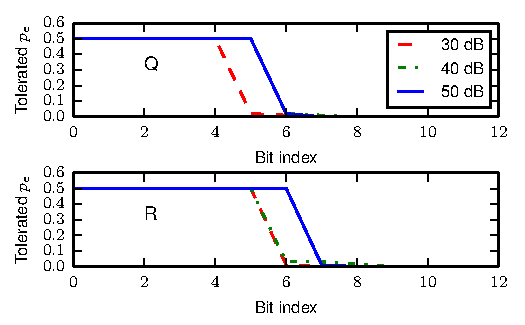
\includegraphics[width=.5\textwidth]{figs/metrics_qr}
  \caption{Tolerable imprecision of a QR decomposition, part of a 8x8 MIMO zero-forcing equalizer, for different signal qualities and a target BER=$0.01$}
  \label{fig:metrics_qr}
\end{figure}
For the second application, the sobel filter, we can see similar results. The output bits correspond to a 32-bit IEEE 754 floating-point number. Many bits of the mantissa can be ignored, which is again dependent on that specific application. Exponent bits can never be pruned. In case of \emph{fdiv} and \emph{fmul} the dynamics are very large, which will result in many approximations at hardware level. In case of \emph{fsqrt}, the possible approximations are independent on the target QoS.
\begin{figure}[tb]
  \centering
  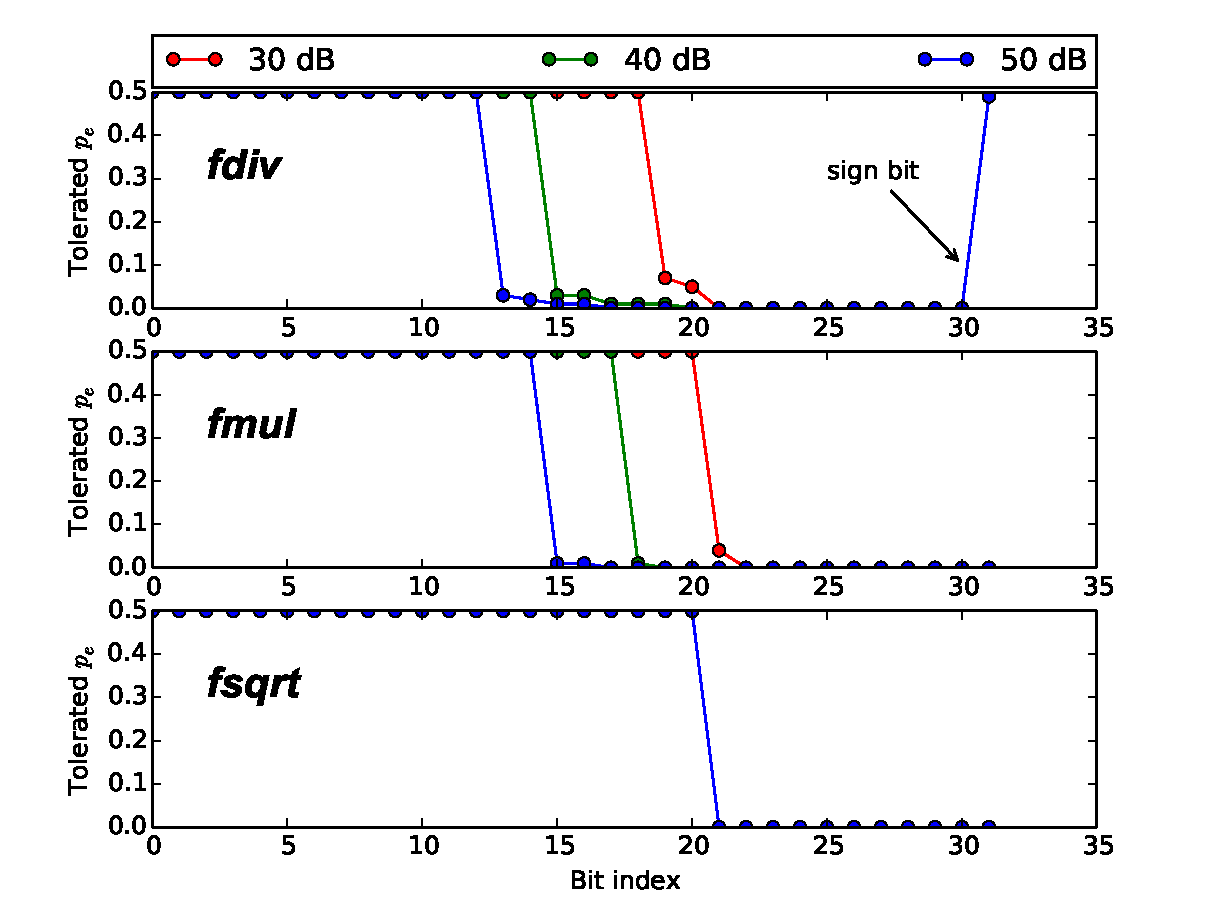
\includegraphics[width=.5\textwidth]{figs/metrics_sobel}
  \caption{Tolerable imprecision of a \emph{sobel} filter for different target qualities (PSNR)}
  \label{fig:metrics_sobel}
\end{figure}


\subsection{Approximation of Sequential Circuits}
\label{subsec:approximation}
With the information generated at the algorithm level, one can now start with the actual hardware approximation. We now know what error probabilities can be tolerated at the circuit output pins for a given required application quality. The next step is to find out which registers in the circuit can be approximated, without violating the constraint. Hence, we are going one step down in the hierarchy. At first, it seemed that the difficulty of performing this step is to find out the one approximation combination that saves most power from a large set off possible approximations. This is why we started solving this problem using evolutionary algorithms, as it can be formulated as a global optimization problem. However, it pointed out not to be the best way. First of all it pointed out to be very unreliable due to the stochastic nature of our problem, as the same set of error applied probabilities leads to different results. Even though they are small, these differences sometimes pushed the algorithms in the wrong direction. And second, the run-time was very long, despite the FPGA-accelerated emulation. The methodology we then came up with consists of 4 steps. With each step we are eliminating approximation candidates. This makes the final, fine-grained approximation step manageable concerning its complexity.
\subsubsection{Data-path Separation}
The first step can be seen as a separation of data- and control-path. The idea is to simply exclude all registers from our potential candidates, that have an influence on outputs, where no errors can be tolerated at all. Influencing means that if there is any path from a register to an output, a fault at that register can also be visible at that output. As these outputs are usually control outputs, like address pins, we call this operation data-path separation. This step has to be performed very careful, as every error in the control-path of a circuit, even if it is very unlikely, can have disastrous effects on the functionality of a circuit. The identification of control path-registers is pretty straight-forward. We subsequently inject into each register an error probability of $p_e=0.5$ but only at one at a time, and observe the outputs. If faults could be observed at at least one unwanted output, this register is discarded from the candidates. In order to make this approach prone to false decisions, it ideally has to be performed several times, with a large set of test-vectors.
\subsubsection{High Variance Registers}
\label{subsubsec:high_v}
The second step pointed out to be in particular necessary in case of the approximation of test circuit ``QR''. We observed that the same set of applied error probabilities resulted in a highly varying output error probability. Although the errors could only be observed at data-path outputs, this behavior makes it impossible to reliably approximate a circuit. In order to trust the approximation, the results have to be reproducable, which is why these elements have to be excluded from the list of candidates as well. We are doing this using the same method as for the data-path separation, but this time we are calculating the variance over multiple runs. If the variance is above a certain threshold the register will be discarded.
\subsubsection{Coarse-grained Approximation}
The third step is the first approximation step. In this step we are identifying those registers that can be completely pruned. As a consequence, all elements prior to that, that only influence that one register can be pruned as well. Hence, this is the step that will save most power in the end. As we have excluded all inappropriate elements in the previous steps, this step is straightforward, as shown in Algorithm \ref{alg:coarse_approximation}. The subset of candidates is denoted as the vector $\mathbf{c} = \{c_1,c_2,\ldots,c_{o}\}$.
\begin{algorithm}
  \caption{Coarse Approximation}\label{alg:coarse_approximation}
  \begin{algorithmic}[1]
    \Procedure{CoarseApproximation}{$\mathbf{c},\mathbf{p_{e,max}}$}
    \For{$i\gets 1,o$}
    \State $\mathbf{p_e(i)} \gets 0.0$
    \EndFor

    \For{$i\gets 1, o$}
    \State $\mathbf{p_e}(c_i) \gets 0.5$
    \State $\mathbf{p_{e,outputs}}$ = injectFaults($\mathbf{p_e}$)
    \If {$\mathbf{p_{e,outputs}} > \mathbf{p_{e,max}}$}
    \State $\mathbf{p_e}(c_i) \gets 0.0$
    \Else
    \State AppendToArray($\mathbf{c_{coarse}},i$)
    \EndIf
    \EndFor
    \State \textbf{return} $\mathbf{p_{e,coarse}} \gets \mathbf{p_e}$
    \EndProcedure
  \end{algorithmic}
\end{algorithm}
We are simply ``switching off'', i.e. injecting faults with an error probability of $p_e=0.5$, one register by another and check whether the output error constraint is violated or not. If it is, we switch back on that register, and continue with the next one. Due to the large error probability of the injected faults, this step can usually be performed very fast. Only a few million cycles have to be emulated in order to get a reliable result.
\subsubsection{Fine-grained Approximation}
Finally, the last step is the fine-grained approximation. In this step we want to find out which error probability, other than $0.5$, can be tolerated at the circuit registers. We are step-wise raising the applied error probabilities to see if the required constraint is still satisfied. There are two main alternatives in approaching the approximation limit. One is to make the approximation at individual registers as high as possible. The other is to approximate evenly over the registers. If a register is holding data from a large combinational logic block it might be beneficial to tolerate as much approximation as possible. However, we think that tolerating a small approximation at many locations is favorable. Previous work has shown that by tolerating a small error probability, large power savings can be made in logic gates, due to an exponential correlation \cite{korkmaz2006advocating}, which is a clear argument for the second approach. Furthermore, in the former case, usually the whole precision budget is consumed by very few registers, which would limit the significance of this step. At this point it would be possible to use complex optimization algorithms to find the optimal distribution of register precision. However, as mentioned earlier, fur us it pointed out to bring no further improvement. Additionally, due to the first three steps our search-space is already highly sorted-out, so that we can simply iterate over the set of candidates, as shown in Algorithm \ref{alg:fine_approximation}. 
\begin{algorithm}
  \caption{Fine Approximation}\label{alg:fine_approximation}
  \begin{algorithmic}[1]
    \Procedure{FineApproximation}{$\mathbf{c},\mathbf{c_{coarse}},\mathbf{p_{e,max}},\delta$}
    \State $\mathbf{c_{fine}} = \mathbf{c} \setminus \mathbf{c_{coarse}}$\Comment{Finding the relative complement}
    \State $\mathbf{p_e}(\mathbf{c}) \gets 0.0$
    \State $\mathbf{p_e}(\mathbf{c_{coarse}}) \gets 0.5$
    \While{(!isEmpty($\mathbf{c_{fine}}$))}
    \For{$i\gets 1, \textrm{numel}(\mathbf{c_{fine}})$}
    \State $\mathbf{p_e}(c_{\textrm{fine},i}) \gets \mathbf{p_e}(c_{\textrm{fine},i}) + \delta$
    \State $\mathbf{p_{e,outputs}}$ = injectFaults($\mathbf{p_e}$)
    \If {$\mathbf{p_{e,outputs}} > \mathbf{p_{e,max}}$}
    \State $\mathbf{p_e}(c_{\textrm{fine},i}) \gets \mathbf{p_e}(c_{\textrm{fine},i}) - \delta$
    \State removeFromArray($\mathbf{c_{fine}},i$)
    \EndIf
    \EndFor
    \EndWhile
    \State \textbf{return} $\mathbf{p_{e,approximation}}$ = $\mathbf{p_e}$
    \EndProcedure
  \end{algorithmic}
\end{algorithm}
The injected error probability of each candidate gets increased step by step by a factor of $\delta$. If the increase led to a constraint violation this particular register is removed from the candidates. This procedure is continued until the set is empty. The result of this operation is a vector containing the maximum error probability for each register in the circuit, where a value of $0.5$ corresponds to coarse-grained approximated registers and other values to fine-grained approximated registers.
\section{Experimental Results}
\label{sec:experimental_results}
In this section we present the experimental results of our proposes methodology. Additional to the two applications presented in Subsection \ref{subsec:application_reasoned}, we introduce a third benchmark, a \emph{Viterbi} decoder. The precision dynamics do come in this case again due to varying signal qualities. However, the major difference to e.g. the MIMO (QR) benchmark is, that the output of the decoder practically has to be error free. For instance in case of digital audio broadcast (DAB), a frame would be discarded if the checksum of the viterbi output is wrong, resulting in an immediate sound drop. A summary of the circuits is shown in Table \ref{tab:benchmark_circuits}.
\begin{table}[htb]
%\renewcommand{\arraystretch}{1.3}
\caption{The benchmark circuits used for this evaluation}
\label{tab:benchmark_circuits}
\centering
\begin{tabular} {| l | l | c | c | c |}
\hline
Name & Description  & Flip-flops & Technology\\
\hline\hline
fpu100 \cite{al2007fpu100} & 32-bit floating point unit  & xx & Synopsys 90nm\\
QR \cite{gimmler-dumont_asic_2013} & QR decomposition  & 414 & Virtex 6\\
vitdec \cite{fehrenz2014viterbi} & Viterbi decoder (131,81)  & 1297 & Virtex 6\\
\hline
\end{tabular}
\end{table}


\subsection{Approximation Evaluation}
We start by evaluating the approximation itself. We want to verify if the methodology allows to efficiently approximate circuits.
% and if the approximation approaches precisely a desired target precision. 
Figure~\ref{fig:optimization_qr} and Table \ref{tab:approx} are showing the approximation for benchark circuit ``QR''. 
\begin{figure}[htb]
  \centering
  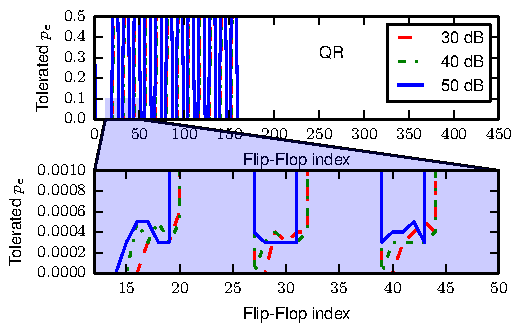
\includegraphics[width=.5\textwidth]{figs/optimization_qr}
  \caption{Approximation result for benchmark circuit ``QR'', showing the maximum tolerable error probability at each register}
  \label{fig:optimization_qr}
\end{figure}
One can see that only a subset of the registers was qualified for approximation. Actually only the ``R'' part could be approximated. Although the algorithm was able to detected registers influencing the ``Q'' part, all have been filtered out in step \ref{subsubsec:high_v}. Only those registers influencing the ``R'' part, have a predictable coherence between error probability at the register and the measured error probabilities at the outputs. However for the remaining elements an approximation was possible. One can see that the one bit reduction of precision, for a signal quality of $50$dB, at application level, spreads over multiple registers at register level. Furthermore, one can see that the fine-grained approximation is also working well. The better the signal quality, the more faults can be tolerated.
The results of benchmark circuit ``fpu'' are similar. The sum of tolerated error probabilities over all registers is shown in Table \ref{tab:approx}. This time the emulated target technology is an ASIC implemented in Synopsys 90nm technology. As we have already seen at application level, one can see that the possible approximations vary a lot depending on the target quality. This will have a clear impact on the power consumption, as we will see in the Subsection~\ref{subsec:power}.
\begin{table}[htb]
\caption{Possible Approximation for benchmark circuit \emph{QR} and \emph{fpu100} for different quality goals}
\label{tab:approx}
\centering
\begin{tabular} { l  l  l  l  l }
\multicolumn{2}{l}{QR} & & \multicolumn{2}{l}{fpu100} \\
\cline{1-2} \cline{4-5}
Signal Qual. [SNR] & $\sum p_{e,i,\textrm{max}}$ & & Target Qual. [PSNR] & $\sum p_{e,i,\textrm{max}}$\\
\cline{1-2} \cline{4-5}
30 dB & 36.5183 & &50 dB & 214.5132 \\
40 dB & 36.519 & &30 dB & 207.0054 \\
50 dB & 42.5191 & &20 dB & 187.0082 \\

\hline



\end{tabular}
\end{table}
%\begin{figure}[htb]
%  \centering
%  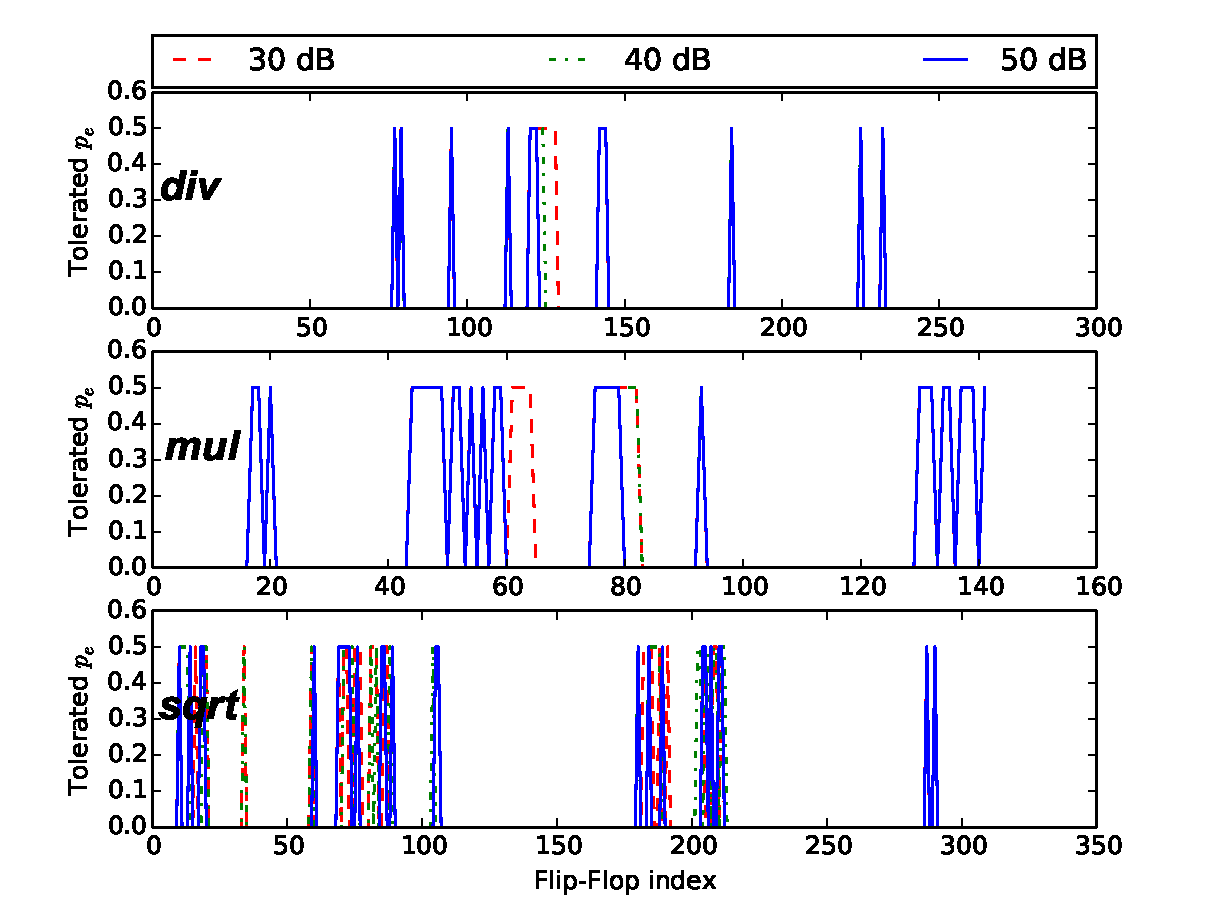
\includegraphics[width=.5\textwidth]{figs/optimization_fpu}
%  \caption{Approximation result for benchmark circuit ``fpu''}
%  \label{fig:optimization_fpu}
%\end{figure}

And finally, Figure \ref{fig:power_viterbi} is showing the results of the approximation of the viterbi decoder. The Figure is showing the sum of tolerable error probabilities over all registers depending on the signal quality. This circuit offers no dynamics in case of coarse-grained approximations. I.e. no parts of the circuit can be switched off and on depending on the signal quality. However, in case of the fine-grained approximation the algorithm was able to find a corresponding working point for each signal quality. Hence, this circuit is in particular useful for approximate computing through voltage over-scaling.
\begin{figure}[htb]
  \centering
  % \showthe\columnwidth
  % \missingfigure[figwidth=.5\textwidth]{Power viterbi}
  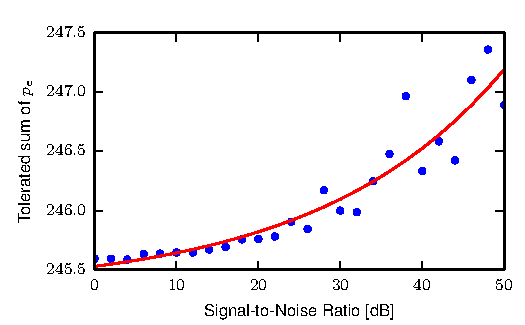
\includegraphics[width=.5\textwidth]{figs/optimization_viterbi}
  \caption{Possible approximation, in terms of tolerated error proabilities, for benchmark circuit ``viterbi'' for varying signal qualities and a target BER=$0.0$}
  \label{fig:power_viterbi}
\end{figure}


\subsection{Power Evaluation}
In this section we are evaluating the power savings enabled by the approximation presented in the previous Sections. We are only able to estimate the power savings enabled by circuit pruning. In order to estimate the power savings enabled by voltage scaling one would need an estimate of the connection between supply voltage and error probability due to timing violations. This is a complex topic on its own, which we keep open for our future work. Figure \ref{subsec:power} is showing the estimated dynamic power consumption of test circuit \emph{QR}. 
\label{subsec:power}
\begin{figure}[htb]
  \centering
  %\missingfigure[figwidth=.5\textwidth]{Potential Power-savings for benchmar circuit ``QR'' for varying signal qualities}
  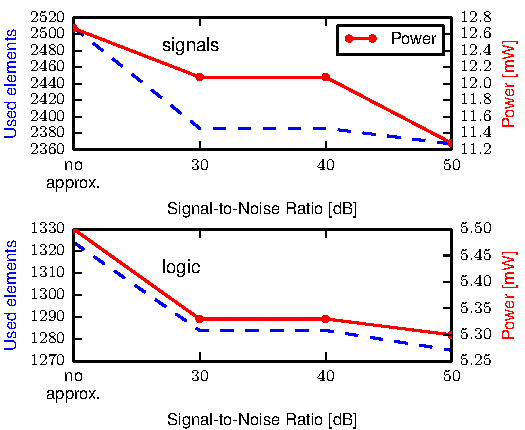
\includegraphics[width=.5\textwidth]{figs/power_qr}
  \caption{Dynamic power consumption of benchmark circuit \emph{QR} for different approximations based on varying signal qualities, when peforming 8x8 ZF Equalization}
  \label{fig:power_qr}
\end{figure}
The power estimations have been made for a Virtex 6 FPGA. One can see that compared to the deterministic original circuit, up to $1,6$ mW can be saved depending on the signal quality. An increase of the signal qualtity from $30$ to $50$ dB can save $0.83$ mW of power.
Figure \ref{fig:power_fpu} is showing the estimated power consumption of test circuit \emph{fpu100}. The power is estimated using the Synopsys 90nm generic library. Compared to the deterministic version up to xx mW can be saved.
\begin{figure}[htb]
  \centering
  %\missingfigure[figwidth=.5\textwidth]{Power FPU}
  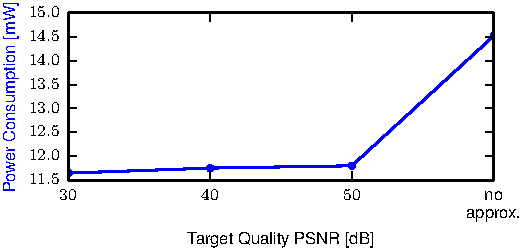
\includegraphics[width=.5\textwidth]{figs/power_fpu}
  \caption{Power consumption of benchmark circuit \emph{fpu100} for different approximations based on varying target qualities, when performing a sobel filter}
  \label{fig:power_fpu}
\end{figure}






\section{Conclusion}
\label{sec:conclusion}






%\section*{Acknowledgment}
%This work was partly supported by the German Research Foundation (DFG) as part of the Transregional Collaborative Research Centre ”Invasive Computing” (SFB/TR 89) and by the German Federal Ministry of Education and Research (BMBF) under grant number 16M3091F.




% trigger a \newpage just before the given reference
% number - used to balance the columns on the last page
% adjust value as needed - may need to be readjusted if
% the document is modified later
%\IEEEtriggeratref{8}
% The "triggered" command can be changed if desired:
%\IEEEtriggercmd{\enlargethispage{-5in}}

% references section
\bibliographystyle{IEEEtran}
\bibliography{IEEEabrv,islped}





% that's all folks
\end{document}
